\section{Scalar multiplication}

\begin{outcome}
\begin{enumerate}
\item[A.] Multiply a scalar by a vector algebraically and geometrically.
\item[B.] Use the laws of scalar multiplication to prove equalities
  between vector expressions.
\end{enumerate}
\end{outcome}

Scalar multiplication of vectors in $\R^n$ is defined as 
follows.

\begin{definition}{Scalar multiplication of vectors in $\R^n$}{vectorscalarmultiplication}
  If $k\in\R$ is a scalar and $\vect{u}\in \R^{n}$ is a vector, then
  their
  \textbf{scalar multiplication}\index{vector!scalar multiplication}
  $k\vect{u}\in \R^{n}$ is defined by
  \begin{equation*}
    k\vect{u}=k\begin{mymatrix}{c}
      u_{1} \\
      \vdots \\
      u_{n}
    \end{mymatrix} = \begin{mymatrix}{c}
      ku_{1} \\
      \vdots \\
      ku_{n}
    \end{mymatrix}.
  \end{equation*}
\end{definition}

For example $3 \mat{ 1, 2, 3 }^T = \mat{ 3, 6, 9 }^T$ and
$-2\mat{ 1, 2, 3 }^T = \mat{ -2, -4, -6 }^T$.

\begin{example}{Geometric meaning of scalar multiplication}{geo-scalar-mult}
  Let $\vect{u}=\mat{2,1}^T$, and draw the following vectors to scale:
  $2\vect{u}$, $\vect{u}$, $\frac{1}{2}\vect{u}$, $0\vect{u}$,
  $-\frac{1}{2}\vect{u}$, $-\vect{u}$, and $-2\vect{u}$.  What is the
  geometric meaning of scalar multiplication?
\end{example}

\begin{solution}
  Here is a picture of the seven vectors. We draw their tails in
  different places to make their relationship easier to see.
  \begin{center}
    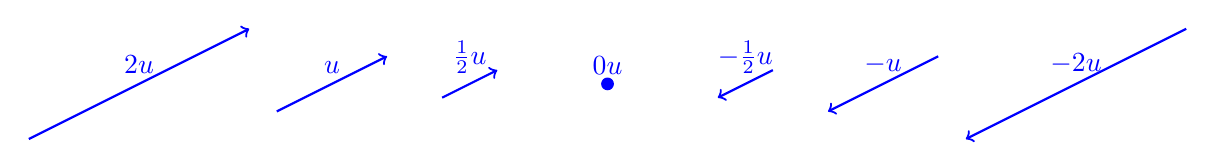
\begin{tikzpicture}[scale=0.7]
      \draw[->, thick, blue] (-10.5,-1)    -- node[above]{$2\vect{u}$} +(4,2);
      \draw[->, thick, blue] (-6,-0.5)  -- node[above]{$\vect{u}$} +(2,1);
      \draw[->, thick, blue] (-3,-0.25) -- node[above]{$\frac{1}{2}\vect{u}$} +(1,0.5);
      \draw[fill, blue](0,0) circle [radius=3pt] node[above]{$0\vect{u}$};
      \draw[->, thick, blue] (3,0.25)   -- node[above]{$-\frac{1}{2}\vect{u}$} +(-1,-0.5);
      \draw[->, thick, blue] (6,0.5)    -- node[above]{$-\vect{u}$} +(-2,-1);
      \draw[->, thick, blue] (10.5,1)      -- node[above]{$-2\vect{u}$} +(-4,-2);
    \end{tikzpicture}
  \end{center}
  We see that the vector $k\vect{u}$ has the same direction as
  $\vect{u}$ when $k$ is positive, and the opposite direction when $k$
  is negative. Further, the length of the vector is scaled by a factor
  of $\abs{k}$. It increases if $\abs{k}>1$ and decreases if
  $\abs{k}<1$. For example, the vector $2\vect{u}$ is exactly twice as
  long as $\vect{u}$.  (It is because of this scaling property that
  scalars are called scalars\index{scalar!for scaling}).
\end{solution}

Just as with addition, scalar multiplication of vectors satisfies
several important properties. These are outlined in the following
theorem.

\begin{theorem}{Properties of scalar multiplication}{vectorscalarmult}
The following properties hold for vectors $\vect{u},\vect{v}\in \R^{n}$ and $k,p $
scalars.
\begin{itemize}
\item The Distributive Law over Vector Addition
\begin{equation*}
k \tup{\vect{u}+\vect{v}} = k\vect{u}+ k\vect{v}
\end{equation*}
\item The Distributive Law over Scalar Addition
\begin{equation*}
\tup{k + p  }\vect{u} = k \vect{u}+p \vect{u}
\end{equation*}
\item The Associative Law for Scalar Multiplication
\begin{equation*}
k \tup{p \vect{u}} = \tup{k p }\vect{u}
\end{equation*}
\item Rule for Multiplication by $1$
\begin{equation*}
1\vect{u}=\vect{u}  
\end{equation*}
\end{itemize}
\end{theorem}

\begin{proof}
We will show the proof of: 
\begin{equation*}
k \tup{\vect{u}+\vect{v}} = k \vect{u}+ k \vect{v}.
\end{equation*}
Assume $\vect{u}=\mat{u_{1},\ldots,u_{n}}^T$ and
$\vect{v}=\mat{v_{1},\ldots,v_{n}}^T$. We have:
\begin{equation*}
\begin{array}{ll}
k \tup{\vect{u}+\vect{v}} & =k \mat{u_{1}+v_{1},\ldots,u_{n}+v_{n}}^T \\
& = \mat{k \tup{u_{1}+v_{1}}, \ldots, k \tup{u_{n}+v_{n}} }^T \\
& = \mat{k u_{1}+ k  v_{1}, \ldots, k u_{n}+ k v_{n}}^T \\
& = \mat{k u_{1}, \ldots, k u_{n} }^T + \mat{k v_{1}, \ldots, k v_{n} }^T \\
& = k \vect{u}+k \vect{v}.
\end{array}
\end{equation*}
\end{proof}

